% Chapter 1
\section*{Preface}
In this chapter, a brief description has been made on the parameters required for understanding a battery performance and various types of batteries available in current market.
\pagebreak
\chapter{Batteries --- an introduction} % Main chapter title
 \label{chap1} % For referencing the chapter elsewhere, use \ref{Chapter1} 
%----------------------------------------------------------------------------------------
% Define some commands to keep the formatting separated from the content 
\newcommand{\keyword}[1]{\textbf{#1}}
\newcommand{\tabhead}[1]{\textbf{#1}}
\newcommand{\code}[1]{\texttt{#1}}
\newcommand{\file}[1]{\texttt{\bfseries#1}}
\newcommand{\option}[1]{\texttt{\itshape#1}}

%----------------------------------------------------------------------------------------
According to International Energy Agency's (IEA) estimate, 5.67 x 1020 joules of energy was produced and used in 2013, equivalent to about 18.0 terawatt-hour (TWh). One TWh is equivalent to 1 billion tons of coal per year, which was the earth's entire energy consumption in 1890. The world is switching to renewable technologies. People are now powering their houses by tapping solar energy , by installing solar panels on their rooftops. However, solar and wind energy have variable output. The sun doesn't always shine and wind doesn't always blow. Energy storage is a necessity for a continuous supply of power. It also provides a more stable and flexible grid system. Batteries store energy in a chemical form and this energy can be used at a later time. If used in houses, a battery can store the power generated by the sun for several hours. In a grid system, when supply is higher than demand, electricity can be used to power storage devices. When demand is higher than supply, stored energy can be used by the grid. To understand how a battery works, it is important that we understand a few terms that are helpful in evaluating its performance. 

\begin{figure}[tbh!]
\centering
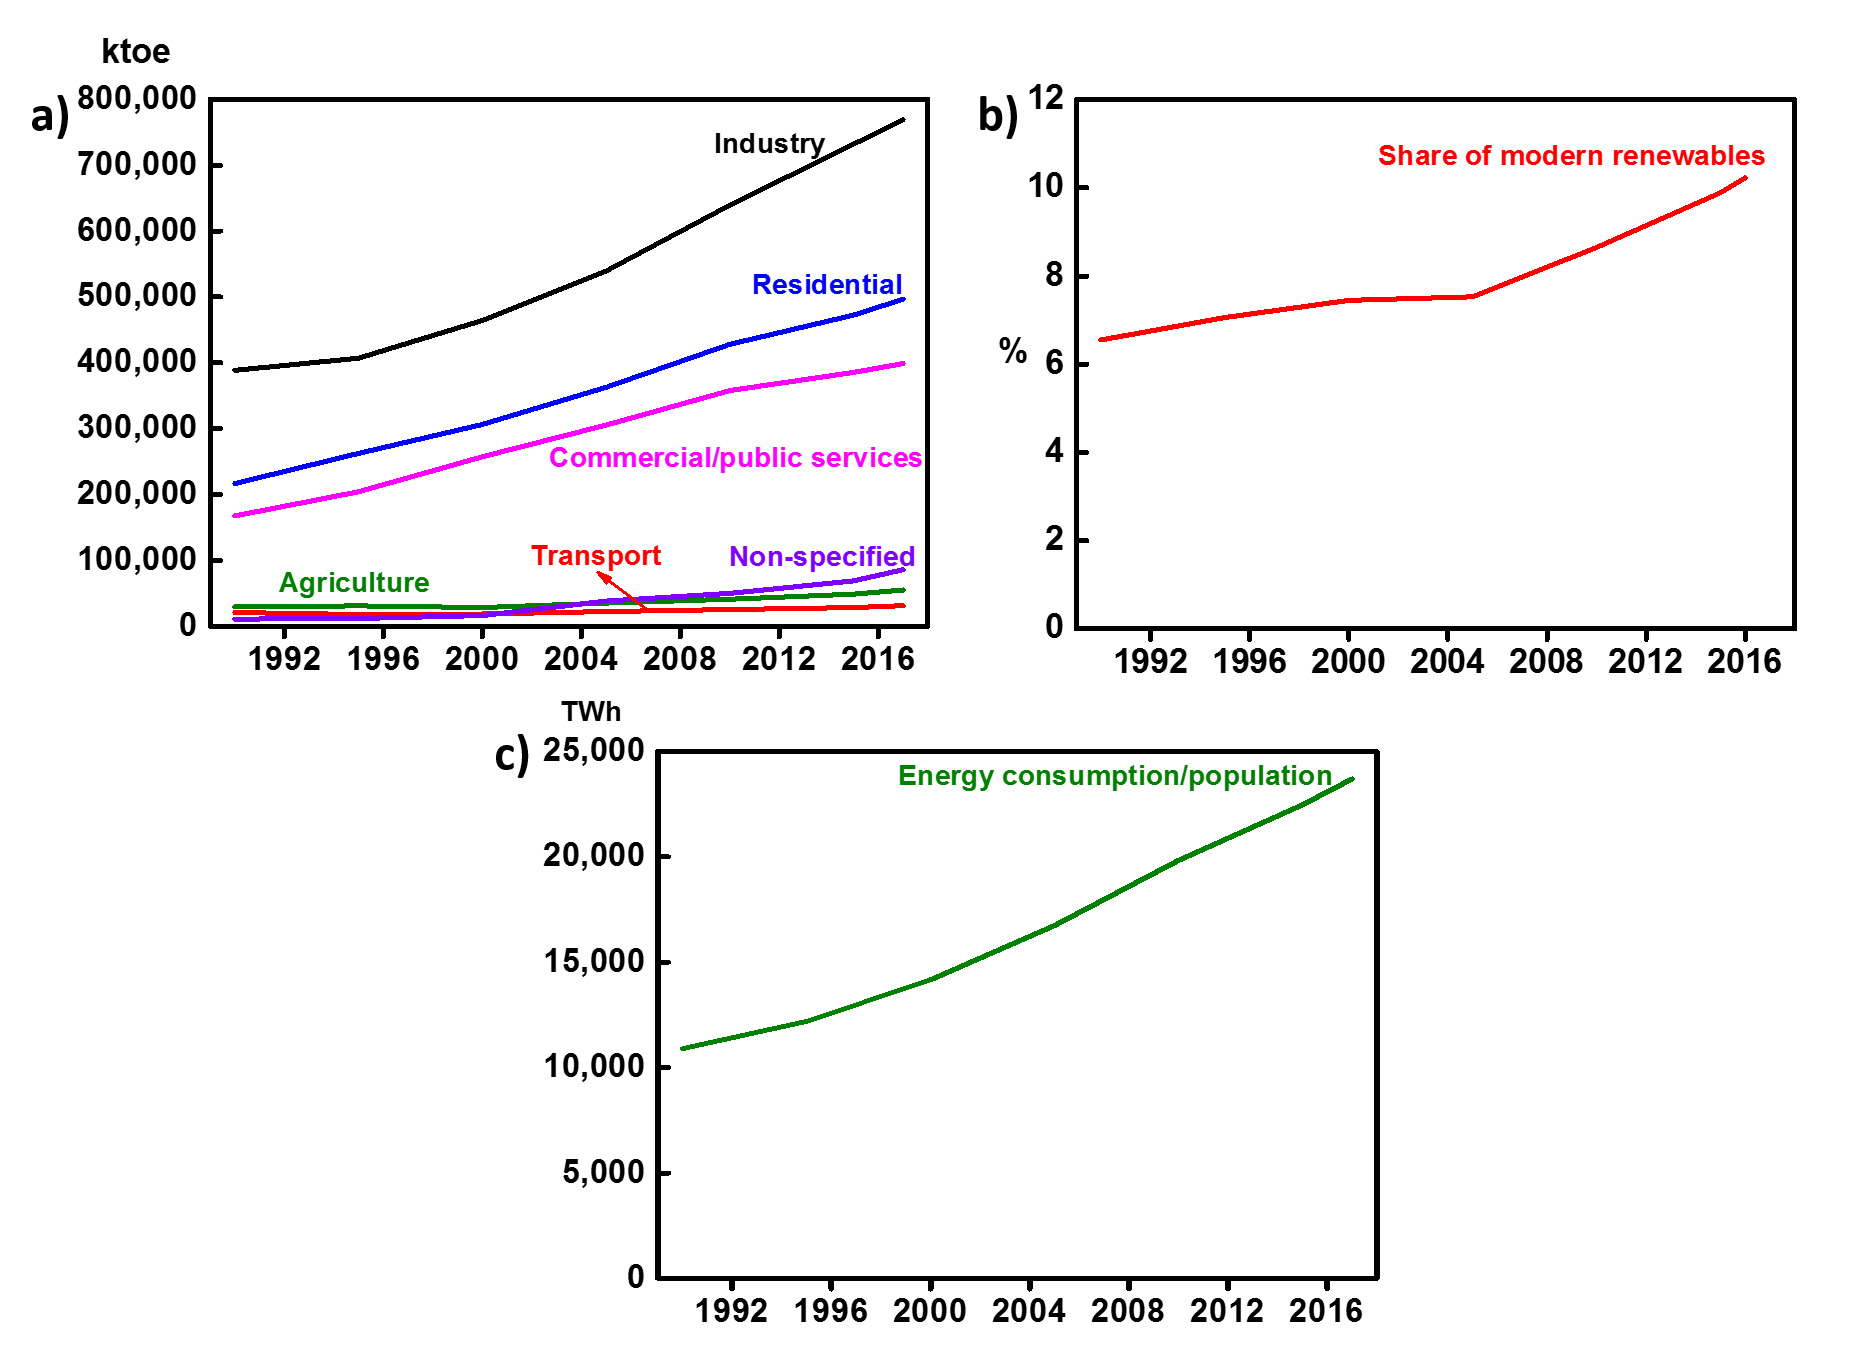
\includegraphics[width=\textwidth]{Figures/chap1fig/IECdata}
\caption{Based on IEA data from the IEA (2018) Monthly Oil Data Service, www.iea.org/statistics. All rights reserved.}
\label{Figures/chap1fig:IECdata}
\end{figure}

\begin{itemize}
\item \textbf{Battery capacity}: Capacity is the amount of charge or energy stored in a battery. Mathematically, it is evaluated by integrating current over time. The fundamental units of battery capacity is coulombs (C), though Amp-hrs (Ah) is more commonly used.  Theoretical capacity (ideal capacity under equilibrium conditions) is calculated with the help of chemical reactions that take place inside the cell. Using Faraday’s constant (F = 96,484.56 C mol$^{-1}$), total available charge in a battery ot its capacity can be determined using equation:

\begin{equation} \label{eq1}
  \text{Capacity(Ah)}=\frac{n \times F \times 1 \text{ hour}}{3600 \text{ sec}}
\end{equation}

\item \textbf{Battery potential}: Voltage is the  most important characteristic of a battery. It is the point usually in the middle of a discharge curve. This is where voltage stays for the longest period during discharge forming a plateau. Various factors help determine a cell's voltage such as electrolyte stability, polarization of the battery and concentrations of the active species. Figure \ref{Figures/chap1fig:CDCforcellvoltage} represents an ideal charge/ discharge curve (CDC). To avoid any permanent damage, a battery should not be discharged below a certain level. This voltage is called the "cut-off voltage". Going beyond a cut-off might lead to certain reactions that decompose the electrolyte (also called side reactions) resulting in an irreversible capacity loss. 

\begin{figure}[tbh!]
\centering
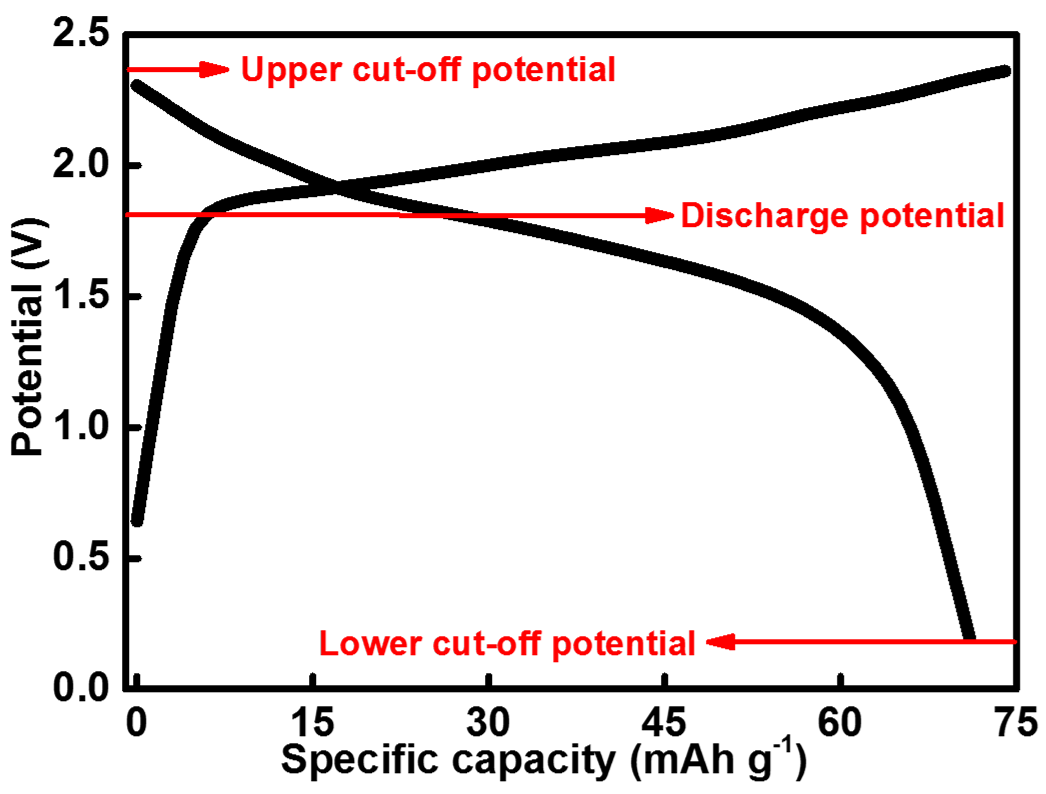
\includegraphics[width=0.8\textwidth]{Figures/chap1fig/CDCforcellvoltage}
\caption{A charge/ discharge curve of an aluminium ion cell using graphite as the cathode and pure aluminium as the anode. The cell was charged and discharged to 2.45 V and 0.2 V respectively.}
\label{Figures/chap1fig:CDCforcellvoltage}
\end{figure}

\item \textbf{Energy density}: The amount of energy stored in a given system per unit mass or volume is called the energy density of a battery. primary function of a battery is to store electrical energy. Heavy batteries are required to move something as large as a car over long distances, therefore they use batteries with high energy density. A simple way to determine the specific energy or energy density of a battery is using Eq.\ref{eq2}:

\begin{equation} \label{eq2}
    \text{Energy density}= \text{Battery capacity (Ah)} \times \text{Battery voltage (V)}
\end{equation}

\item \textbf{Power density}: Power density measures how quickly a battery can deliver energy. Also known as specific power, it's equivalent to the maximum current one can draw from a battery. Units used to describe power density are W kg$^{-1}$ or W m$^{-3}$. The best way to differentiate between energy and power density of a battery is to use an example of a moving car. Energy density determines how 'far' the car will go, whereas power density determines how 'fast' the car will go.

\item \textbf{Coulombic efficiency}: Coulombic efficiency of a battery is the ratio of number of charges that enter during charge to the number that can be extracted from the battery during discharge.  A high coulombic efficiency in excess of 95\% is considered a standard value for commercial battery systems. Any loss in coulombic efficiency can be attributed to some secondary reaction (side reactions) in the battery system. 
\end{itemize}

\textbf{Primary and secondary batteries}: Primary or non-rechargeable batteries produce current immediately when assembled. They have very high energy densities since it is a single-use system. Implanted medical devices, guided missiles, mars rovers and military ordnance use primary batteries. They prove to be an uneconomical energy source since they produce only about 2\% of the power used during their production. Common types of disposable batteries include zinc–carbon and alkaline batteries. 
\textit{Secondary}, or rechargeable batteries, need to be charged before their first use. Since they are  assembled in the discharged state, applying an electric current (during charge) reverses the cell's active materials chemical state. They find extensive use in portable devices as they store energy reversibly. The oldest form of rechargeable battery is the lead–acid battery, which has been used since the 1700's. These batteries find extensive use in automotive, power tools, laptop computers, mobile phones, toys, etc. The most commonly used examples of rechargeable batteries are lithium-ion batteries, nickel-cadmium (NiCad) and nickel metal hydride (NiMH) batteries. 

The charging/discharging rates affect the rated battery capacity. If the battery is being discharged very quickly (high discharge current is applied), then amount of energy that can be extracted from the battery is reduced and its capacity decreases. This is because only a fraction of the total reactants are converted to other forms, and therefore the energy available is reduced. Alternately, if a battery is discharged using low current, more energy can be extracted from the battery and the battery capacity is higher. The temperature of a battery also affects the energy that can be extracted. At a higher temperature, the battery capacity is typically higher than at a lower temperature. However, intentionally elevating battery temperature is not an effective method to increase battery capacity as this also decreases battery lifetime. 
An ideal battery should be low-cost, get charged and discharged indefinitely under high or low current rate, have a long lifetime with high coulombic efficiency (>95\%), and low-self discharge. However, it is difficult to fulfil the above set of requirements. Researchers are building batteries that might achieve these objectives \cite{. 

\section{Current rechargeable batteries}

\subsection{Lead-acid batteries}
These batteries are the most commonly used in photovoltaic systems. A battery is made of pure lead and lead oxide (\ce{PbO2}) electrodes to store energy and aqueous sulfuric acid is used as electrolyte. The battery has a long lifetime and is cheap compared to other battery types. However, the batteries have a low energy density, only moderate efficiency and high maintenance requirements. Both lead and sulfuric acid are  hazardous materials, which makes a lead-acid battery quite unsafe to use. 

\subsection{Nickel-cadmium (NiCad)}
Nickel-cadmium may be cost effective on a life-cycle/cost basis. They consist of a positive electrode of nickel (or hydroxide) and a negative electrode of cadmium hydroxide. They are commonly used in a sealed configuration in small household appliances. NiCad batteries have several advantages such as a long lifetime and long storage life. The redox processes occur on the surface of the electrodes which means there is no loss of the active material. These processes increase the cell's lifetime. Furthermore, the electrolyte in nickel-cadmium is less corrosive to battery parts than in a lead-acid battery which also increases lifetime. A NiCad cell can be fully discharged and charged without damaging the battery. NiCad batteries are less sensitive to colder temperature, tolerating temperatures of -50$^{\circ}$C. In addition, the NiCad batteries have low maintenance requirements. Unlike, lead-acid batteries, NiCad batteries do not use corrosive elements and require less frequent maintenance. However, they also have a number of disadvantages. Some of the disadvantages include; Expense. Nickel-cadmium batteries are typically at least twice as expensive than lead-acid batteries and record lower coulombic efficiencies between 75\% to 85\%.

\subsection{Vanadium redox-flow batteries}
 Redox flow batteries use a reduction-oxidation between two valence states in solution rather than changing the composition, and hence the valence states of solid material on an electrode. A flow battery consists of two volumes of solution separated by a selective membrane which allows some ions to pass but not others. Flow batteries have several potential advantages over solid batteries. A key advantage, which is particularly important in transport applications, is that the battery may be re-charged simply by pumping out the uncharged solution and replacing the solution with charged solution. This eliminates potentially long recharging times, such as are encountered in electric vehicles. Replacement of the solution allows the electric car to be recharged in the same fashion in which a car is filled with fuel. Another advantage is that the capacity of the battery is determined by the volume of solution, while the power of the battery is determined by the membrane contact area between the two solutions. The vanadium-Vanadium redox flow battery, developed at the University of New South Wales, is a particularly promising flow battery. It consists of two states of Vanadium. It has high efficiencies, with coulombic efficiencies of 97\% and energy efficiencies of 87\%. In addition, since both solutions (anode and cathode) in the battery use vanadium, cross contamination between the two solutions may discharge the battery, but will not cause damage to the battery.
 
\subsection{Lithium and lithium-ion battery (LIB)}
An electrochemical potential is a measure of the energy of the outer most electrons. Examination of the electronic configuration of the outer shell of the material gives an indication of the magnitude and sign of the electrochemical potential between the reactants and products of a redox reaction taking place inside a battery. The standard potential of a redox reaction is used to determine if a redox reaction will occur spontaneously (if it will generate a voltage between the reduction and oxidation reaction). If the difference between the standard potentials is positive, then the reaction will proceed spontaneously. If the standard potential is negative, a voltage needs to be applied in order for the reaction to proceed, which is precisely what is needed in a battery. Therefore, standard potential is an important parameter to find a suitable battery anode. Lithium has the highest electrochemical potential. It can achieve very high energy and power densities in high power battery applications. Many variations (such as lithium-ion) of the basic lithium chemistry have been developed for specific applications. Lithium is a highly flammable metal. Early commercial cells with metallic lithium cathodes were considered unsafe because of this property. However, modern cells use compounds of lithium that do not react as aggressively. A typical Li-ion cell use graphite for its anode and lithium-cobalt dioxide (LiCoO$_2$) or a lithium-manganese compound (\ce{LiMnO4}, \ce{Li2MnO3}) as cathodes. An electrolyte is a medium that allows ion-transfer inside the cell. The most commonly used electrolyte for LIBs is based on \ce{LiPF6} and mixtures of cyclic and linear carbonate solvents. The linear carbonates, such as dimethyl carbonate (DMC), ethyl methyl carbonate (EMC), or diethyl carbonate (DEC), maintain low viscosity of the electrolyte and enhance its conductivity. However, they are flammable and show flash points around room temperature (between 16 and 33$^{\circ}$C). In combination with an oxidant and an ignition source, they may catch fire and cause explosions. Using non-flammable electrolyte solvents or of flame-retardant electrolyte additives enhances the safety of flammable electrolytes, it deteriorates the electrochemical performance of batteries. 
The lithium-ion battery system is a power pack of choice not only on the Earth, but also in space. Last year in October, a few astronauts on board the International Space Station (ISS) stepped outside their quarters for a spacewalk. Flight engineers Christina Koch and Jessica Meir (first all female spacewalk) were assigned the task of manually swapping out two nickel hydrogen (NiH) batteries for one brand new lithium-ion battery (LIB). This would not only upgrade the station's complex electrical system but also extend it's life through 2020's. ISS was launched into orbit in 1998 with 48 NiH batteries. The National Aeronautics and Space Administration (NASA) has started swapping these old batteries, since 2017, with 24 new LIBs  that provide higher energy density and a better power efficiency. Naturally, they had to be careful while handling these heavy batteries (195 kg). LIBs come with a potential risk of \textit{thermal runaway}- defects or manhandling a battery to overheat and explode. Inside a pressurised oxygen-rich capsule, the results would have been catastrophic! 
However, LIBs have become the leading pioneers in battery technology especially for portable consumer electronics. Additionally, volume production has brought the prices down.

\section{Aluminium-ion battery}
To find a suitable battery system, one needs to examine theoretical specific capacities of different ions that can replace lithium, using \ref{eq1}. Metals in the upper left corner of the periodic table, such as sodium (Na), magnesium (Mg), potassium (K) and calcium (Ca) reported higher theoretical capacities than the others and can be alternatively used as battery anodes. Table  \ref{table1} shows calculations for a few common metal anodes. 

\begin{table}[tbh!]
\caption{Comparing important parameters of various metal anodes.} \label{table1}
\begin{tabular}{lccccrr}
\headrow
\hline
 & \textbf{Li} & \textbf{Na} & \textbf{Mg} & \textbf{Al} & \textbf{K} & \textbf{Ca}\\
\hline
Valence electrons & 1 & 1 & 2 & 3 & 1 & 2\\
Specific capacity (mAh g$^{-1}$) & 3862 & 1166 & 2205 & 2980 & 685 & 1340\\
Standard potential (V) & -3.04 & -2.71 & -2.36  & -1.68 & -2.93 & -2.87\\
Abundance (ppm) & 18 & 22700 & 23000 & 82000 & 18400 & 41000\\
\hline  % Please only put a hline at the end of the table
\end{tabular}
\end{table}

Table \ref{table1} shows lithium to be one of the most promising candidates. An important drawback with lithium is that it is rare. Lithium and cobalt have been exhaustively used in the LIB industry and we might run out of these resources after 25-30 years. The second most promising metal is aluminium (Al), which has a relatively high standard oxidation potential. Aluminium-ion batteries (AIBs) using aluminium metal as anode will be cost-effective, easily recyclable, and much safer to use than LIBs.  In Na-ion and LIBs, a monovalent ion is intercalated/ deintercalated into/from the electrode compared to a trivalent ion in AIBs. Since three charges are involved in the redox reactions, a higher specific capacity and energy density might be obtained. The electrolyte is a chemical medium that allows the flow of charge between the cathode and anode. It acts like a catalyst by promoting the movement of ions from the cathode to the anode. The electrolyte of a battery is usually made of soluble salts, acids or other bases in liquid, gelled or dry media; it might be a polymer (in LIBs), soil or concrete (Zn-ion batteries), or ionic liquids, also known as molten salts (in AIBs). The electrolyte is there to put the different chemicals of the anode and cathode into contact with one another, in a way that the chemical potential can equilibrate from one terminal to the other, converting stored chemical energy into useful electrical energy. The ions transport current through the electrolyte while the electrons flow in the external circuit generating an electric current. 

\subsection{Aqueous aluminium-ion batteries (AAIBs)}
Using water instead of organic solvents or ionic liquids as an electrolyte would reduce the battery costs significantly and increase battery safety.
However, these batteries come with their own set of problems. 
\begin{itemize}
    \item the electrochemical plating/stripping of aluminium occurs at a
    voltage far from the stable potential window of water
    \item \ce{AlCl3}, which is used in the electrolyte, is highly acidic and sometimes results in dissolution of active material and corrosion of battery parts
    \item No cathode material has yet been reported with a good cycling stability 
\end{itemize}  
Anatase titanium oxide (\ce{TiO2}) has been investigated as intercalation (insertion of a molecule or ion) electrodes. \ce{TiO2} nanostructures have been commonly used as cathode materials in aqueous AIBs. Using black \ce{TiO2} nanoleaves, He \textit{et al.} achieved a capacity of 271 mAh g$^{-1}$, while \ce{TiO2} nanospheres produced a capacity of 180 mAh g$^{-1}$ over 30 cycles. Improving characteristics such as cycle life, efficiency and rate capability would enable these batteries to be used for high power applications such as regenerative braking or high power grid services.However, limited focus has been given to cycle life, efficiency and rate capability in the recent aqueous Al-ion literature. Cycling data for \ce{TiO2} nanotubes were presented up to cycle 13 by Liu et al \cite{liu_aluminum_2012}.  Recently, a graphene enhanced \ce{TiO2} electrode was shown to produce a capacity between 10 and 25 mAh g$^{-1}$ at a current density of 6.25 A g$^{-1}$. However, only 125 cycles were possible and coulombic efficiency was observed to be very low at approximately 50\%. Similarly, the charge discharge profiles observed for the nanospheres and nanotubes show low coulombic efficiencies of around 80-85\%. The reason for low efficiency of \ce{TiO2} in aqueous AIB electrolyte is yet to be explored, but the possibilities could be oxidation of \ce{Ti3+} due to dissolved \ce{O2} in electrolyte, \ce{H2} gas evolution or an irreversible reduction of \ce{Ti4+} to \ce{Ti2+} while charge.  
Aluminium in aqueous or protic systems forms a passivating oxide film as well as metal corrosion. At standard conditions, it instantaneously forms a very thin (thickness $\sim$2–10 nm), uniform, and continuous amorphous surface layer of \ce{Al2O3} \cite{vargel2004translated}. This oxide film is stable over a pH range of about 4.0–8.6. Although this would be an advantage when using aluminium anode in LIB cathode \cite{myung_electrochemical_2011}, it provides a barrier for solvation of aluminum and transportation of \ce{Al3+}, which poses a big challenge for using Al metal directly as anode.

\subsection{Non-aqueous AIBs}
Rechargeable AIBs emerge as a competitive alternative post-lithium batteries. As typical multi-electron reaction devices, AIBs possess the potential of higher specific capacity, superior volumetric energy density, and comparable gravimetric energy density to lithium-ion batteries6,8,9. Moreover, the high abundance and easy accessibility of Al resources enable Al-ion batteries to become an ideal candidate for large-scale energy storage system9. Because the standard electrode potential of Al$^{3+}$/Al (−1.68 V) is lower than \ce{H+}/\ce{H2}, the evolution of \ce{H2} occurs due to the reaction between aluminum foil and aqueous acid or alkali solution. Thus, Al cannot be electrochemically striped or deposited in a common aqueous solution. To be compatible with Al anode, the ionic liquid \ce{AlCl3}/[EMIM]Cl with a wider range of electrochemical active window emerges as the typical electrolyte, which provides a mild corrosive effect on the Al surface to activate the Al striping and plating reaction. However, such type of ionic liquid electrolytes are not preferable for the application in large-scale energy storage systems due to its high cost and potential environmental concerns. Therefore, an alternative nonflammable and low-toxicity aqueous electrolytes for low-cost rechargeable aluminum-ion battery is urgently needed. Another critical issue that limits the application of Al batteries is the low energy density due to the lack of proper cathode materials. Thus far, there are two categories of cathode materials for rechargeable Al batteries. One is the carbon-based materials with high specific surface area such as 3D graphite-foam that can accommodate AlxCly − 12–18. Owing to the ultra-fast monovalent reaction kinetics18, the 3D graphite-foam delivers a high power density of 3000 W kg$^{−1}$. At the same time, the monovalent reaction inherently limits the obtainable specific capacity. Among the carbon-based materials, the highest reported specific capacity (graphene nanoribbons on highly porous 3D-graphene foam) was only 148 mAh g$^{−1}$, which is far from practical requirements. The other category of cathode materials can realize trivalent reaction and thus have the potential to achieve high specific capacity, but they suffer from relatively lower redox potentials. It is well known that the strong electrostatic nature of \ce{Al^{3+}} always leads to sluggish kinetics, high over-potentials, and the eventual collapse of host structure. Therefore, to accommodate trivalent \ce{Al^{3+}}, it is essential for the cathode materials to possess weak bond strengths between the host frameworks (namely, moderate polarity). The representatives with moderate polarity are sulfur, transition metal sulfides, Prussian blue analogues, and some transition metal oxide. These materials have promoted a relatively reversible trivalent reaction, but with discharge voltages only ranging from 0.3 to 0.8 V can hardly be considered as valid cathode materials. As such, there is an urgent need for the development of cathode materials for Al batteries with high capacity and high redox potential.

\subsection{Cathodes in non-aqueous AIBs}
Chloroaluminates have been known for aluminium electrodeposition since the 1970s and have also been used as electrolytes for rechargeable aluminium batteries. Systems with a general formula MCl-\ce{AlCl3} where \ce{M+} can be a cation like \ce{Na+}, \ce{Li+} or an organic species like pyrrolidinium or immidazolium have been tested as electrolytes for rechargeable AIBs. These melts can be acidic, basic or neutral. In the acidic systems, the dominant species is \ce{Al2Cl7^{-}}, while in a basic system \ce{Cl-} and \ce{AlCl4^{-}} anions coexist whereas in neutral melts, only \ce{AlCl4^{-}} anions exist. A usable cathode material should have certain properties- good conductivity, high A number of criteria is considered before selecting a battery electrode. The most important ones being natural. A good battery cathode is stable in the presence of an electrolyte, deliver a good working voltage, a large reversible storage capacity should be obtained at that potential and the electrode should be easy to fabricate. 
Theoretical capacity of a material can be found using :

\begin{equation} \label{eq3}
    C_{t}= \frac{n \times F}{3.6 \times M}
\end{equation}\\
where n = number of reactive electrons per formula unit,\\
M = molar weight of the material and\\
F = Faraday constant\\

The formula denotes that a material with low molecular weight and high number of reactive electrons would deliver a high theoretical capacity.

\begin{figure}[h!]
\centering
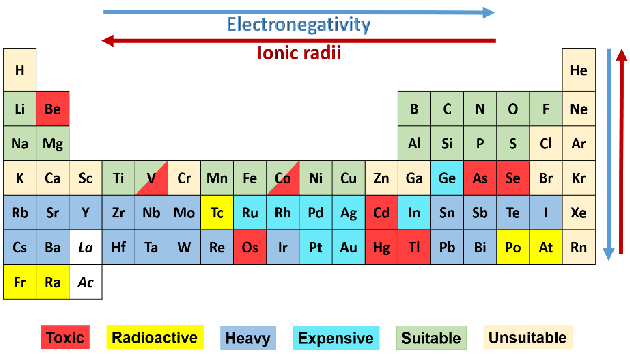
\includegraphics[width=\textwidth]{Figures/chap1fig/pertab}
\caption{The periodic table suggesting elements that can be used as battery materials. However, a few elements from this table have shown good electrochemical performance such as Mo, Sn, Nb and W. Potassium and calcium-ion batteries have also been studied.}
\label{Figures/chap1fig:pertab}
\end{figure}

Figure X displays the elements that can be used for designing new cathodes. However, some transition metals such as V or Co, despite their toxicity, have been tried and tested. Transition metals have variable valence states; this increases the number of electrons that can be stored, increasing the battery capacity. The type of bond formed between a metal ion and the ligand plays an important role in determining the electrochemical potential of the material. When the electronegativity difference between the two is high, an ionic bond is formed. A smaller difference results in a covalent bond. Materials with a covalent bonds form poorly packed structures, while ionic bonds form dense structures. A stable structure would enhances the phase stability and electrochemical potential of the material \cite{melot}. Furthermore, electrode potential depends on the ionic radius of the material. When an atomic nuclei is loosely bound to its valence electrons, the system needs lower energy for electron transfer , which leads to a lower potential. If more energy is consumed during electron transfer (materials that have a lower ionic radii), the electrochemical potential of the material increases. using equation:

\begin{equation} \label{eq4}
    -\Delta G = n \times F \times E
\end{equation}\\
where $\Delta$G = change in internal energy during ion intercalation,\\
n = number of electrons stored per formula unit,\\
F = Faraday constant and\\
E = electrochemical potential of the material.\\

Therefore, the electr
\section{Research objectives}

The goal of this PhD project is to find new cathodes for rechargeable AIBs that perform better than state-of-the-art. 
\begin{itemize}
    \item Materials that have a layered structure, such as graphite, allow intercalation of charge-carrying species when the cells charge and discharge. We propose that materials with a similar structure, such as molybdenum dichalcogenides, a few transition metal oxides or sulfides, boron nitride (inorganic graphite) would undergo a similar mechanism and deliver a stable performance. 
    
    \item Materials with high surface area such as activated carbon or nano-structured materials, provide a better contact between the cathode and the electrolyte, thus have proven to be good battery materials. They provide a faster and an efficient pathway for electron diffusion, which improves the kinetics of the system and increases the battery's energy density. We tested high surface-area materials such as activated carbon, carbon black, nanostructures of molybdenum dichalcogenides, as cathodes for non-aqueous AIBs to confirm our hypothesis.
    
    \item Once a cathode achieves high capacity (> 60 mAh g$^{-1}$), and a high voltage (> 1.0 V), it is equally important to establish its mechanism. This would help in designing a better cathode. X-ray diffraction studies, Raman spectroscopy, and X-ray photoelectron spectroscopy are a few techniques that have been used to analyse cathode materials. 

\end{itemize}






